Wykorzystując zaproponowany model możemy zaprojektować elementy optyczne do koncentracji promieniowania elektromagnetycznego. Takie mikrourządzenia można zbudować wykorzystując zarówno struktury płaskie jak przedstawiona na rysunku \ref{fig:old-concen-eps} i rys.~\ref{fig:old-concen-pow}, jak i~cylindryczne rys.\ref{fig:concen-cyl}, czy też zbudowane z~kilku elementów typu core-shell \ref{fig:concen-core-shell}
\begin{figure}[!htb]
	\centering
	\begin{subfigure}[b]{.45\textwidth}
		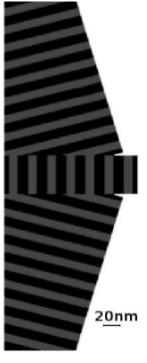
\includegraphics[angle=90,width=\textwidth]{images/multilayer/konc_eps_mgr.png}
		\caption{Struktura warstwowa do koncentracji promieniowania E-M}
		\label{fig:old-concen-eps}
	\end{subfigure}
	\begin{subfigure}[b]{.45\textwidth}
		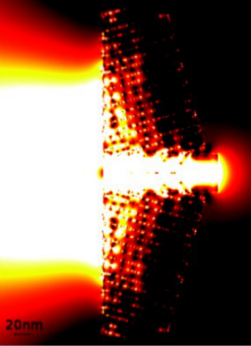
\includegraphics[angle=90,width=\textwidth]{images/multilayer/konc_ene_mgr.png}
		\caption{Rozkład energii pola E-M wewnątrz koncentratora na rysunku (a)}
		\label{fig:old-concen-pow}
	\end{subfigure}

	\begin{subfigure}{.45\textwidth}
		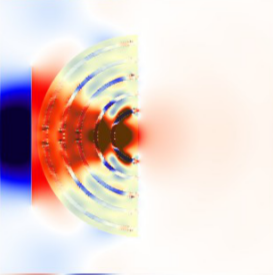
\includegraphics[width=\textwidth]{images/multilayer/konc_polk_poynt.png}
		\caption{Cylindryczny koncentrator promieniowania E-M}
		\label{fig:concen-cyl}
	\end{subfigure}
	\begin{subfigure}{.45\textwidth}
		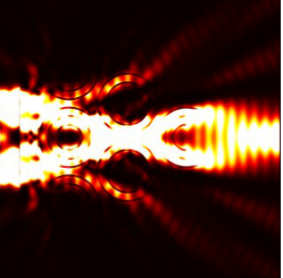
\includegraphics[width=\textwidth]{images/multilayer/konc_coreshell_energy.png}
		\caption{Koncentrator promieniowania E-M oparty na strukturach typu core-shell}
		\label{fig:concen-core-shell}
	\end{subfigure}

	\caption{Wyniki symulacji  metodą FDTD układów do koncentracji promieniowania E-M~\cite{pastuszczak2011slanted}} 
\end{figure}



